\section{Performance details of the track-to-vertex association}
\label{sec:Appendix_TrackVertex}
In this note, a track-to-vertex association method is used that is different from the one
in Ref.~\cite{ATLASConfNote:PUcorrection}. In Ref.~\cite{ATLASConfNote:PUcorrection},
tracks are assigned to vertices by requiring $|\Delta z \times \sin\theta| < 1 \unit{mm}$. 
In cases where more than one vertex satisfied this
criterion, the ambiguity was resolved by choosing the vertex of higher $\sum_{\rm tracks}{p_T^2}$. Here, 
we chose a different approach:
\begin{itemize}
    \item Step 1: The vertex reconstruction is used to associate tracks with vertices. If a track is attached to more than one vertex, priority is given to the vertex with higher $\sum_{\rm tracks}{p_T^2}$. 
    \item Step 2: If a track is not associated with any primary vertex after step 1, but satisfies $|\Delta z|<3~\unit{mm}$ with respect to the hard-scatter primary vertex, it is assigned to the hard-scatter primary vertex. 
\end{itemize}
The second step targets tracks from hadron decays in flight originating from the hard-scatter, which are likely not to be attached to any vertex. 
The $|\Delta z|<3~\unit{mm}$ criteria was chosen based on the $|z_0|$ distribution of tracks from b-hadron decays, but no strong dependence of the performance on the particular criteria was observed when the 
cut value was altered within 1\unit{mm}.
Figure~\ref{fig:ROC_TrkToVtx_corrJVF} and~\ref{fig:ROC_TrkToVtx_RpT} show the efficiency versus fake-rate curves comparing the different track-to-vertex association methods, using a
sample of $20< \pT < 50\GeV$ jets in simulated QCD dijet events. The new method, labelled ``Trk-to-Vtx 3'', shows a significant increase in the hard-scatter jet efficiency at fixed fake rate. 
The large performance gain for b-quark initiated jets is shown in Figures~\ref{fig:ROC_TrkToVtx_corrJVF_b} and~\ref{fig:ROC_TrkToVtx_RpT_b}. 
\begin{figure}[!htbp]
  \centering
  \subfigure[]{
      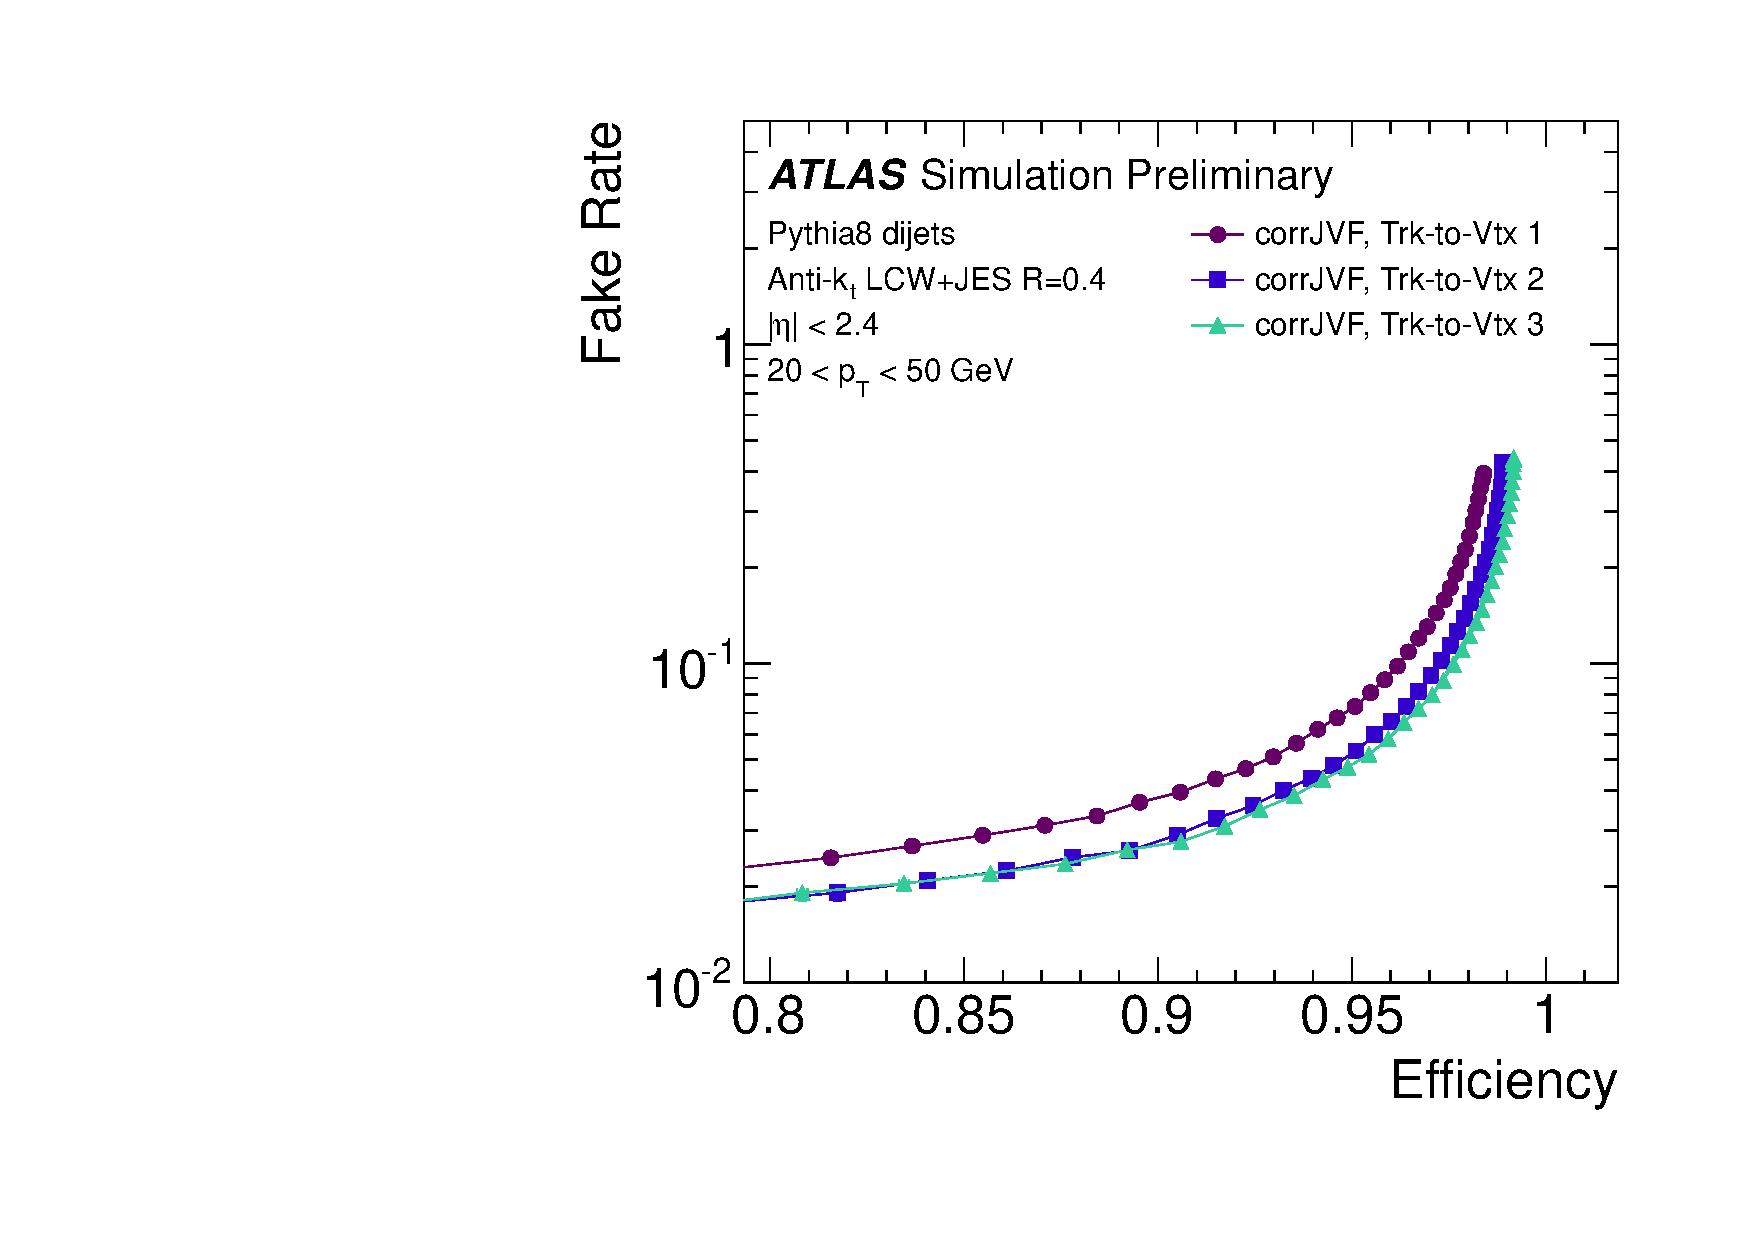
\includegraphics[width= 0.46\textwidth]{ROC_corrJVF_TrkToVtx}
    \label{fig:ROC_TrkToVtx_corrJVF}
  }
  \subfigure[]{
      \includegraphics[width=0.46\textwidth]{ROC_RpT_TrkToVtx}
    \label{fig:ROC_TrkToVtx_RpT}
  }
  \subfigure[]{
      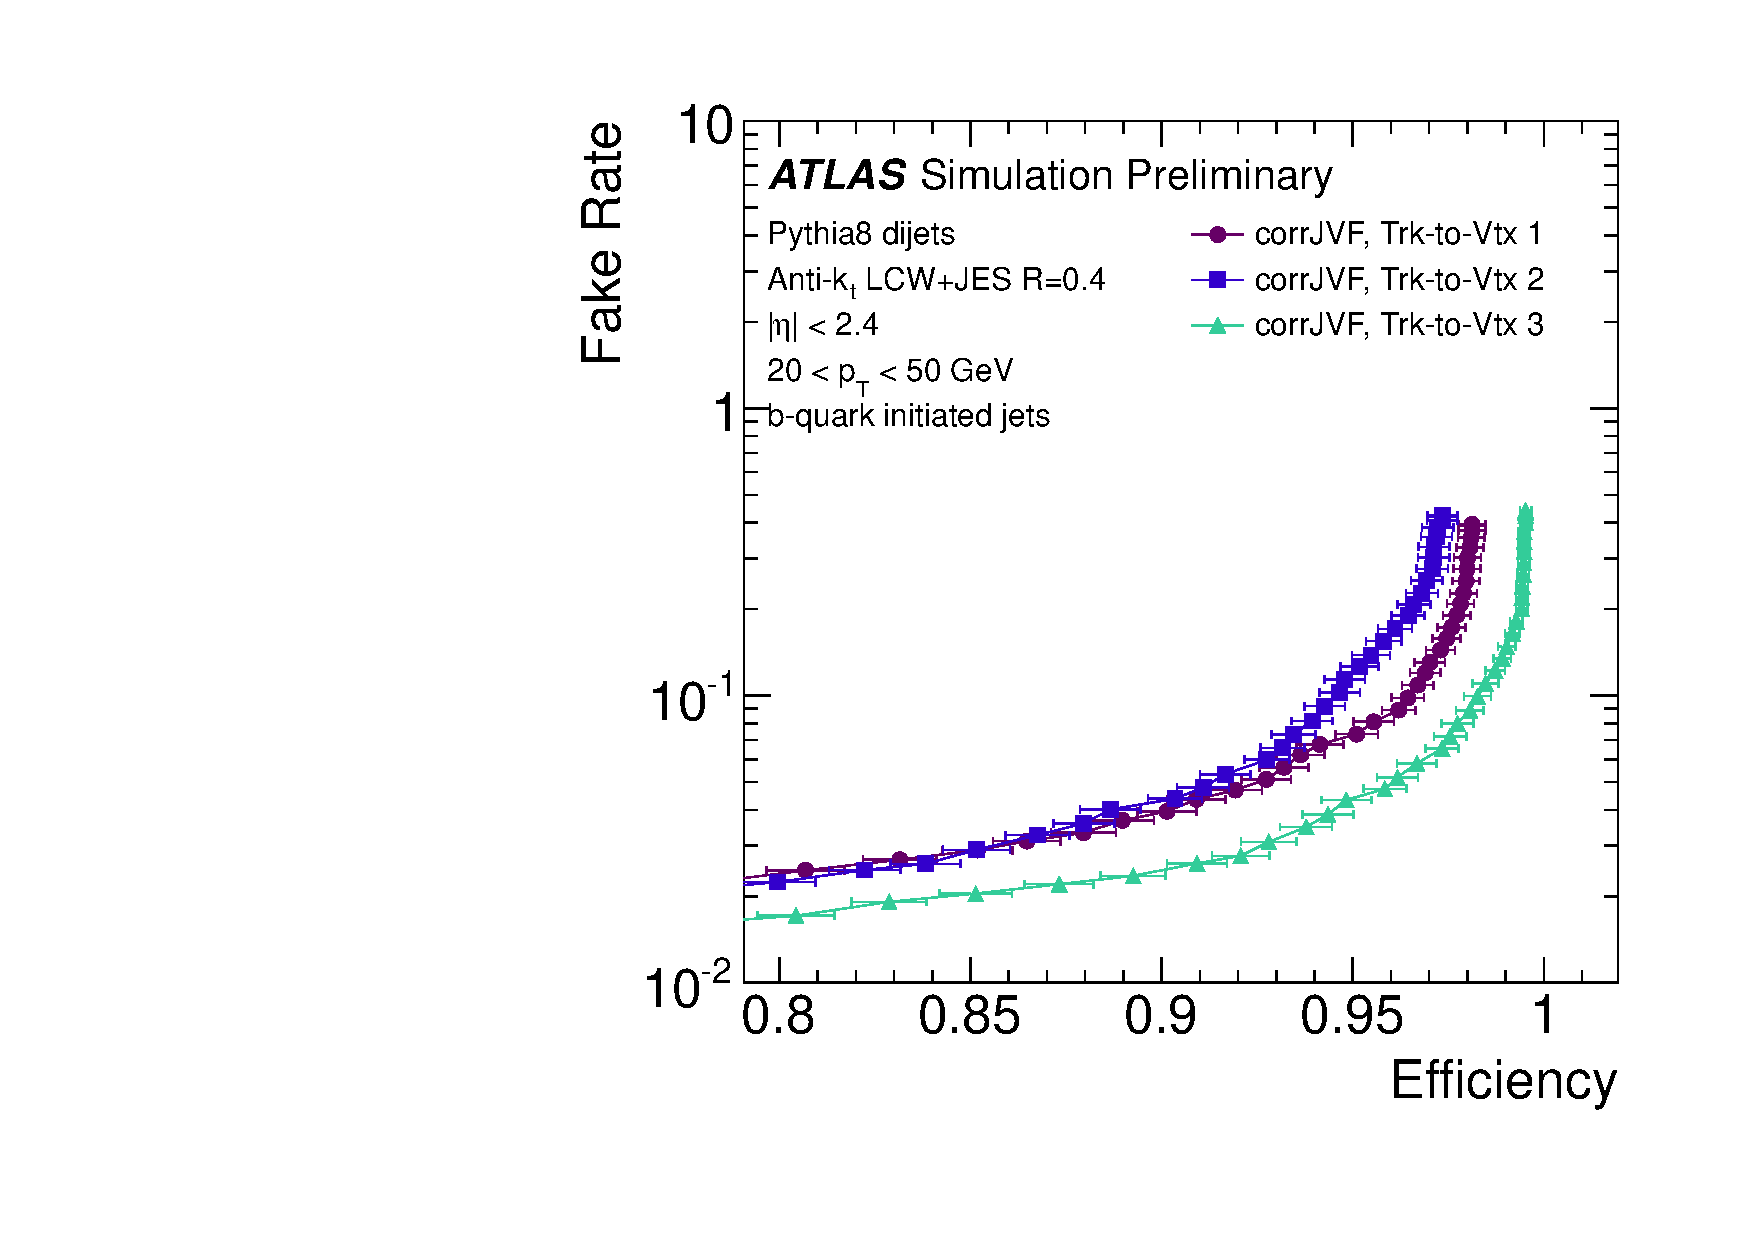
\includegraphics[width= 0.46\textwidth]{ROC_corrJVF_bquark_TrkToVtx}
    \label{fig:ROC_TrkToVtx_corrJVF_b}
  }
  \subfigure[]{
      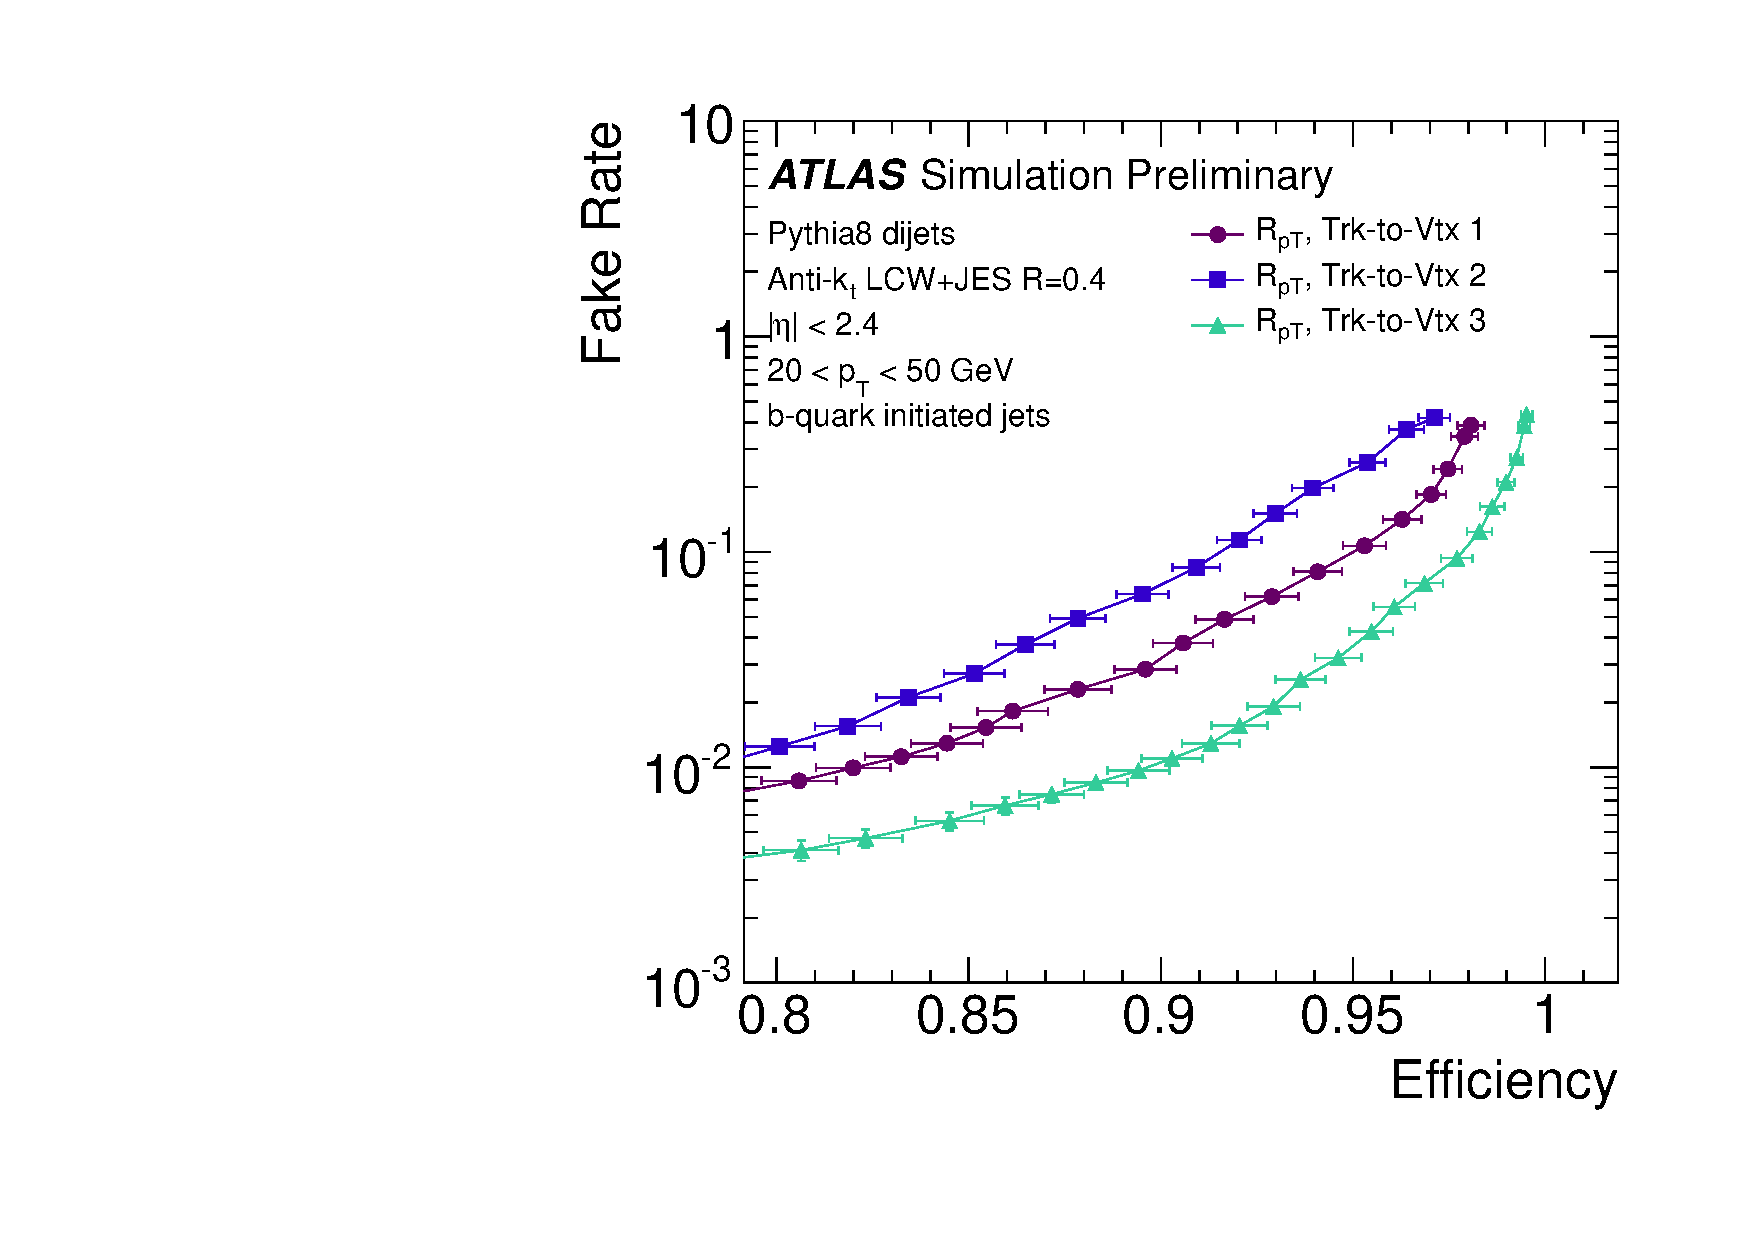
\includegraphics[width=0.46\textwidth]{ROC_RpT_bquark_TrkToVtx}
    \label{fig:ROC_TrkToVtx_RpT_b}
  }
  \caption{Fake-rate versus efficiency curves for \cJVF (a) and \RpT (b) for three different track-to-vertex associations: 
  the ``$|\Delta z \times \sin\theta| < 1 \unit{mm}$'' criteria labeled ``Trk-to-Vtx 1'', ``Step 1'' labelled ``Trk-to-Vtx 2'' and the full new procedure ``Step 1\&2'' labelled ``Trk-to-Vtx 3''.
  For b-quark initiated jets, the performance gain for \cJVF (c) and \RpT (d) of the new method stems from ``Step 2'': without ``Step 2'' the new method would perform worse than the
  ``$|\Delta z \times \sin\theta| < 1 \unit{mm}$'' based association.
  }
\label{fig:test}
\end{figure}
